\documentclass[10pt]{article}
\usepackage[margin=0.9in]{geometry}
\usepackage[utf8]{inputenc}
\PassOptionsToPackage{hyphens}{url}  % let long URLs break at hyphens
\usepackage{amsmath,amssymb,booktabs,graphicx,array,longtable,hyperref,xcolor,natbib,float,caption,rotating}
\hypersetup{colorlinks=true,linkcolor=blue!50!black,citecolor=blue!50!black,urlcolor=blue!50!black}
\graphicspath{{../docs/figures/}}
\newcommand{\accMethod}{36.5\%}
\newcommand{\accCIMethod}{[31.1, 40.9]}
\newcommand{\foneMethod}{0.317}
\newcommand{\coarseMethod}{63.8\%}
\newcommand{\cdMethod}{0.430}
\newcommand{\cdCIMethod}{[0.405, 0.460]}
\newcommand{\nMethod}{312}
\newcommand{\accBone}{32.7\%}
\newcommand{\accCIBone}{[26.3, 40.1]}
\newcommand{\foneBone}{0.276}
\newcommand{\coarseBone}{48.1\%}
\newcommand{\cdBone}{0.400}
\newcommand{\cdCIBone}{[0.335, 0.465]}
\newcommand{\nBone}{156}
\newcommand{\accBtwo}{14.7\%}
\newcommand{\accCIBtwo}{[9.3, 19.9]}
\newcommand{\foneBtwo}{0.146}
\newcommand{\coarseBtwo}{43.6\%}
\newcommand{\cdBtwo}{0.607}
\newcommand{\cdCIBtwo}{[0.563, 0.638]}
\newcommand{\nBtwo}{156}
\newcommand{\accAthree}{36.5\%}
\newcommand{\accCIAthree}{[31.1, 40.9]}
\newcommand{\foneAthree}{0.317}
\newcommand{\coarseAthree}{63.8\%}
\newcommand{\cdAthree}{0.459}
\newcommand{\cdCIAthree}{[0.442, 0.527]}
\newcommand{\nAthree}{312}
\newcommand{\accAfivegaic}{43.3\%}
\newcommand{\accCIAfivegaic}{[37.7, 49.1]}
\newcommand{\foneAfivegaic}{0.380}
\newcommand{\coarseAfivegaic}{65.1\%}
\newcommand{\cdAfivegaic}{0.388}
\newcommand{\cdCIAfivegaic}{[0.349, 0.443]}
\newcommand{\nAfivegaic}{312}
\newcommand{\accBthreea}{7.7\%}
\newcommand{\accCIBthreea}{[4.5, 12.8]}
\newcommand{\foneBthreea}{0.011}
\newcommand{\coarseBthreea}{7.7\%}
\newcommand{\cdBthreea}{0.656}
\newcommand{\cdCIBthreea}{[0.616, 0.706]}
\newcommand{\nBthreea}{156}
\newcommand{\accBthreeb}{7.7\%}
\newcommand{\accCIBthreeb}{[4.5, 12.8]}
\newcommand{\foneBthreeb}{0.011}
\newcommand{\coarseBthreeb}{38.5\%}
\newcommand{\cdBthreeb}{0.679}
\newcommand{\cdCIBthreeb}{[0.630, 0.732]}
\newcommand{\nBthreeb}{156}
\newcommand{\accBthreec}{8.3\%}
\newcommand{\accCIBthreec}{[4.2, 11.9]}
\newcommand{\foneBthreec}{0.079}
\newcommand{\coarseBthreec}{39.1\%}
\newcommand{\cdBthreec}{1.167}
\newcommand{\cdCIBthreec}{[1.059, 1.242]}
\newcommand{\nBthreec}{156}
\newcommand{\estHone}{0.055}
\newcommand{\ciHone}{[-0.021, 0.121]}
\newcommand{\pHone}{0.26}
\newcommand{\estHtwo}{0.030}
\newcommand{\ciHtwo}{[-0.035, 0.091]}
\newcommand{\pHtwo}{0.63}
\newcommand{\estHfivebrefinement}{-0.029}
\newcommand{\ciHfivebrefinement}{[-0.075, -0.017]}
\newcommand{\pHfivebrefinement}{2.9e-28}
\newcommand{\ambiguousFrac}{50.6\%}


\title{Learning to Fit Shapes to Neural Geometry:\\ A Synthetic-Only Shape-Type and Parameter Regressor for Top-3 PCA Activation Clouds}
\author{Libor ``Burny'' Burian}
\date{November 2026}

\begin{document}
\maketitle

\begin{abstract}
Interpretability research repeatedly reports low-dimensional shapes in neural activations: circles for weekdays and months, helices for positions and counts, a paraboloid for colors, lines for temperature and age, polytopes for features in superposition. These shapes are usually identified and fitted by hand. We (i) compile a cited catalog of empirically reported neural geometries, (ii) train a permutation-invariant network \emph{only on synthetic shapes} that maps a 3D point cloud (the top-3 principal components of activations) to one of 13 shape families and to a canonical, unique parameter vector, using a shape-to-shape Chamfer loss against the ground-truth shape plus a point-to-shape residual, and (iii) evaluate it on a preregistered synthetic test set and on real activations of GPT-2, Llama-3.1-8B, a grokked modular-addition transformer and toy models of superposition, against a classical fit-every-family baseline with geometric-AIC model selection, a feature-based classifier, trivial baselines, random controls and inference-time ablations.
% Abstract results sentence; numbers are macros from generated/numbers.tex.
On \nMethod{} held-out synthetic clouds the fitter identifies the family in \accMethod{} of cases; on a shared subset it reaches \accMethodsub{} against \accBone{} for the classical pipeline and \accBtwo{} for the feature classifier, with a lower median Chamfer distance to the ground-truth shape (preregistered H1 and H2 supported). On real activations its coarse shape class agrees with published descriptions on \hthreeAgree{}/\hthreeN{} preregistered datasets, which is not above a permutation null (H3 not supported). Post-hoc inspection points to curves outside the vocabulary, low-variance projections and clouds unlike any training family. Controls show that smooth ordinal processes are often labelled helix, and a preregistered held-out test against the PCA ringing artifact, while necessary, still accepts helix fits on clouds the literature describes as circles.

\end{abstract}

\section{Introduction}
A growing body of work shows that some concepts in language models are represented not by single directions but by low-dimensional manifolds \citep{engels2025notall,bhalla2026sae,gurnee2025linebreaks}. The common workflow is: collect activations for a set of inputs that vary along one concept, project onto the top principal components, look at the 2D/3D scatter, and describe the shape (``a circle'', ``a helix''), often followed by a hand-designed parametric fit \citep{kantamneni2025trig}. This is slow, subjective, and vulnerable to a known artifact: when the similarity between points decays smoothly with an ordinal or latent variable (distance-decaying covariance, random walks, autocorrelated signals), principal component analysis (PCA) yields Fourier-like components and therefore an arch or a helix-like curve in the top components even when nothing ``curved'' is represented \citep{novembre2008horseshoe,diaconis2008horseshoes,antognini2018walks,shinn2023phantom}.

We ask whether the description step can be automated: given the top-3 PCA coordinates of a set of activations, predict which shape family it is and the parameters that uniquely specify the shape, such that the shape passes as close as possible to the points. Our contributions:
\begin{enumerate}
\item A catalog of empirically reported neural geometries with model, layer, method, whether the shape is visible in the top-3 PCs, and verified sources (Sec.~\ref{sec:catalog}).
\item A 13-family shape vocabulary covering the catalog entries that can be represented in 3D, with differentiable samplers, label margins between nested families, and canonical forms that make the output parameters unique (Sec.~\ref{sec:families}), including a family for the PCA ``ringing'' confounder.
\item A Set Transformer fitter trained only on on-the-fly synthetic shapes with domain randomization, a shape-to-shape Chamfer loss, and test-time refinement (Sec.~\ref{sec:method}).
\item A preregistered evaluation (hypotheses H1--H5; H5a needs the postponed trained ablations) on synthetic and real activations with baselines, controls, inference-time ablations, bootstrap confidence intervals and multiple-testing correction (Sec.~\ref{sec:setup}--\ref{sec:results}); both positive and negative results are reported.
\end{enumerate}

\section{Background and related work}
\label{sec:catalog}
\paragraph{Empirical neural geometries.} Circles for days of the week and months were found with sparse-autoencoder feature clusters in GPT-2 and Mistral-7B, and with PCA of hidden states on day and month arithmetic prompts in Mistral-7B and Llama-3-8B \citep{engels2025notall}; GPT-2's learned positional embeddings form a helix in their top-3 PCs \citep{yedidia2023helix}; the character count since the last line break lives on a rippled helix-like curve in Claude 3.5 Haiku \citep{gurnee2025linebreaks}, a finding replicated in Llama-3.1-8B and Qwen3-8B \citep{sinii2026counting}; numbers form a generalized helix \citep{kantamneni2025trig}; Llama-3.1-8B layer 19 shows a paraboloid for colors, a helix for years, a circle for days and lines for temperature and age \citep{bhalla2026sae}; in grokked modular-addition transformers the token embeddings lie on circles, one per key frequency \citep{nanda2023progress,zhong2023clock}, and in the ``pizza'' algorithm the averaged embeddings of input pairs fill the disc inside the circle \citep{zhong2023clock}; features in superposition form uniform polytopes such as antipodal pairs, triangles, pentagons, tetrahedra and square antiprisms \citep{elhage2022tms}; true and false statements separate in the top two principal components \citep{marks2024truth}; supervised MDS recovers circles, lines, clusters and, for cities, a sphere \citep{tiblias2025smds}; the sky positions of stars and constellations form a sphere, though not within the top three PCs \citep{berdnikov2026sky}; in-context graphs reorganize into rings and grids \citep{park2025iclr}; emotion steering vectors arrange approximately on a circle \citep{sun2026valence}. Outside LLMs, grid cells form a torus \citep{gardner2022torus}, head-direction cells a ring (visualised with Isomap, as PCA often fails to show it; \citealp{chaudhuri2019ring}), natural image patches a Klein bottle \citep{carlsson2008klein}. Appendix~\ref{app:catalog} (generated from \texttt{catalog.yaml}) lists all entries.

\paragraph{Primitive fitting.} Deep primitive fitting on CAD point clouds predicts per-point memberships and fits planes, spheres, cylinders and cones with differentiable least squares \citep{li2019spfn}, B-spline patches \citep{sharma2020parsenet} or regressed parameters \citep{yan2021hpnet}; the classical alternative is RANSAC \citep{schnabel2007ransac} with information-criterion model selection \citep{kanatani2004gaic}. These methods target large CAD clouds with several primitives; neural-geometry clouds have one shape, few points (7 weekdays), high noise, families absent from CAD vocabularies (helix, torus, PCA ringing), and come from a PCA projection of a much higher-dimensional space. To our knowledge, no prior work learns shape-type classification plus parameter regression for activation point clouds. The closest are hypothesis-driven supervised MDS, which needs concept labels and has no free shape parameters \citep{tiblias2025smds}, and manifold fitting with cubic or thin-plate splines through concept centroids, whose shape (closed loop, open curve, sheet) is chosen by hand from the known task structure \citep{wurgaft2026manifold}.

\section{Shape vocabulary}
\label{sec:families}
Each family $f$ maps unconstrained raw parameters $\theta$ to a shape $S_f(\theta)\subset\mathbb{R}^3$, posed by a center $c$ and a rotation $R\in SO(3)$ predicted with the continuous 6D representation \citep{zhou2019rotation}. Table~\ref{tab:families} lists the families with their parameters. Each family provides (i) a differentiable dense sampler on a fixed grid with length/area weights, (ii) label margins so that a generated instance is not (nearly) a member of a simpler family at the sample's noise level (e.g.\ an arc's sagitta must exceed $\max(0.1\,\text{chord},3\sigma)$), and (iii) a canonicalization map that selects a unique representative among parameterizations of the same point set (axis signs fixed by the sign of the largest component; rotation about symmetry axes fixed by projecting the first PCA axis, or the second when the first is nearly parallel to the symmetry axis; point sets sorted by their first PCA coordinate, with approximate tie-breaks on the second and third). The \emph{ringing} family $c+\sum_{k=1}^{3}a_k\cos(k\pi s)e_k$ is the shape PCA produces when similarity decays smoothly with an ordinal variable \citep{novembre2008horseshoe,antognini2018walks}, so a helix claim must beat it. The \emph{polytope} family has six templates: the regular triangle, square, pentagon, tetrahedron and octahedron, and the square antiprism, which is uniform but not regular.

\begin{table}[t]
\centering\scriptsize
\caption{The 13 shape families. Local shapes are posed by a center $c$ and a frame $R=(e_1,e_2,e_3)$ unless stated. Canonical forms make the reported parameters unique.}
\label{tab:families}
\begin{tabular}{llll}
\toprule
Family & Local shape & Canonical unique parameters & Anchor \\
\midrule
blob & $\mathrm{diag}(\sigma_1,\sigma_2,\sigma_3)z$, $z\sim\mathcal{N}(0,I)$ & center, axes (signs fixed), $\sigma_1\ge\sigma_2\ge\sigma_3$ & null class \\
clusters & $k\in\{2..6\}$ centroids + spread & centroids sorted lexicographically, spread & true/false \citep{marks2024truth} \\
polytope & regular template (6 subtypes) & subtype, center, circumradius, sorted vertices & superposition \citep{elhage2022tms} \\
line & $tLe_1$, $t\in[-1,1]$ & endpoints & temperature, age \citep{bhalla2026sae} \\
arc & $r(\cos t\,e_1+\sin t\,e_2)$, $|t|\le\Delta/2$ & center, normal, $r$, extent (closed if $\Delta\approx2\pi$) & days, months \citep{engels2025notall} \\
ellipse & $a\cos t\,e_1+b\sin t\,e_2$ & center, normal, major axis, $a\ge b$ & distorted circle \\
helix & $r\cos t\,e_1+r\sin t\,e_2+\frac{pt}{2\pi}e_3$ & axis, $r$, signed pitch $p$, turns, phase & GPT-2 $W_{pos}$ \citep{yedidia2023helix} \\
ringing & $\sum_{k=1}^3 a_k\cos(k\pi s)e_k$ & $a_1,a_2>0$, $a_3$, frame & PCA artifact \citep{novembre2008horseshoe} \\
disc & $\rho(a\cos t\,e_1+b\sin t\,e_2)$ & center, normal, $a\ge b$ & pizza \citep{zhong2023clock} \\
sphere & cap of half-angle $\alpha$ around $e_3$ & center, $r$, pole, $\alpha$ & cities \citep{tiblias2025smds} \\
paraboloid & $z=\frac12(\kappa_1x^2+\kappa_2y^2)$, $|\kappa_2|\le\kappa_1$ & frame, $\kappa_1,\kappa_2$, patch radius & colors \citep{bhalla2026sae} \\
cone & frustum $r(h)=r_0+gh$ around $e_3$ & axis, bottom/top radius, height & anisotropy \citep{ethayarajh2019contextual} \\
torus & $((R+r\cos v)\cos u,(R+r\cos v)\sin u,r\sin v)$ & center, axis, $R$, $r$ & grid cells \citep{gardner2022torus} \\
\bottomrule
\end{tabular}
\end{table}


\section{Method}
\label{sec:method}
\paragraph{Preprocessing.} Synthetic and real clouds pass through the same map: center, project onto the top-3 principal directions, fix axis signs by the sign of the third moment, force a right-handed frame (3D inputs), and divide by the RMS radius. No whitening is applied, so aspect ratios are preserved.

\paragraph{Synthetic data.} Each training step draws fresh shapes for all 13 families from a dedicated seed stream (test and validation streams are disjoint by construction). Nuisances implement domain randomization \citep{tobin2017domain}: $N\in[5,1024]$ log-uniform, relative noise $\sigma\in[0.003,0.15]$ log-uniform (10\% noise-free), anisotropic noise (30\% of samples), non-uniform sampling densities along curves and surfaces, 0--10\% outliers in 30\% of samples, and, with probability 0.25 per family batch, embedding into $\mathbb{R}^D$ ($D\in\{16,64,256\}$) with noise in all $D$ dimensions followed by PCA back to 3D, which reproduces the real pipeline including projection effects and mirrored frames.

\paragraph{Model.} A Set Transformer encoder \citep{lee2019settransformer} (two ISAB blocks with 16 inducing points, PMA pooling, $d=128$, 4 heads, key-padding masks) maps per-point features (xyz and $\log N$) to an embedding; a classification head outputs logits over the 13 families and one MLP head per family outputs its raw parameters.

\paragraph{Loss.} For a sample of family $y$ with ground-truth shape $S^\ast$ and input points $X$,
\begin{equation}
\mathcal{L}=\mathrm{CE}(\ell,y)+\mathrm{CD}\big(S_y(\hat\theta_y),S^\ast\big)+0.5\,\mathrm{Res}\big(X\to S_y(\hat\theta_y)\big)+0.1\,\mathrm{CE}_{\mathrm{sub}}+\lambda(t)\,\mathrm{Aux},
\end{equation}
where CD is the symmetric, length/area-weighted, unsquared Chamfer distance between dense samples of the predicted and of the noise-free ground-truth shape (restricted to its true extent), Res is a Huber ($\delta=0.05$) point-to-shape residual, $\mathrm{CE}_{\mathrm{sub}}$ classifies the number of clusters and the polytope template, and Aux is an annealed axis/scale term $1-(\hat a\cdot a^\ast)^2+|\log\hat s-\log s^\ast|$ whose weight falls linearly from 1 to 0.1 over the first 30\% of the planned steps. The geometric terms are averaged within each family and then over families. Because CD compares point sets it is invariant to every parameter symmetry, so no canonicalization or matching is needed during training. Only the ground-truth family's head receives geometric losses (teacher forcing; SPFN likewise computes its fitting loss with the ground-truth primitive type, \citealp{li2019spfn}). Training uses AdamW (learning rate $3\times10^{-4}$, weight decay $10^{-4}$), label smoothing 0.05, a 2k-step warmup and a cosine schedule; the 110-minute wall-clock budget stopped training before the end of the schedule (steps in the models table, Appendix).

\paragraph{Inference.} The top-3 families are each refined for 300 Adam steps on the two-sided objective $\frac{1}{N}\sum_i d(x_i,S)+0.25\sum_j w_j d(s_j,X)$, initialized by the network (amortized inference followed by optimization, cf.\ \citealp{kolotouros2019spin}); the second term prevents degenerate inflation of radii and extents. The family is selected by the temperature-calibrated classifier \citep{guo2017calibration}; geometric AIC \citep{kanatani2004gaic} and a hybrid rule are ablations. The output is mapped back to PCA coordinates and canonicalized.

\section{Experimental setup}
\label{sec:setup}
\paragraph{Preregistration.} Hypotheses, metrics, analysis plan and falsification criteria were committed before training (\texttt{reports/preregistration.md}); deviations are logged in \texttt{reports/deviations.md}.
\paragraph{Synthetic test set.} 250 samples per cell of 13 families $\times$ 4 point-count bins $\times$ 3 noise bins (39{,}000 clouds) from the \texttt{test} stream. Baselines run on a fixed subset of 20 samples per family and cell; all paired comparisons use that subset.
\paragraph{Baselines.} B1: classical multi-start fit of every family with the same two-sided objective (initial frames: the identity, two axis permutations and a random rotation; k-means for clusters; every polytope template), 61 refinement runs that leave 22 candidates per cloud, and geometric-AIC selection. B2: hand-crafted features (global PCA eigenvalue ratios; mean and spread over local neighbourhoods of the eigenvalue-based linearity, planarity and scattering \citep{weinmann2014features,weinmann2015features}; persistent-homology H0/H1 lifetimes via ripser \citep{tralie2018ripser}; radial and nearest-neighbour statistics) with gradient-boosted trees, then B1's lowest-objective candidate of the predicted family. B3: always blob, always arc (B1's arc fit; the preregistration specified a full circle), random shape.
\paragraph{Ablations.} A1 parameter-space loss (its configuration also drops the residual term), A2 no residual term, A3 no refinement, A4 DeepSets encoder \citep{zaheer2017deepsets}, A5 selection rule, A6 no $\mathbb{R}^D$ augmentation; A1/A2/A4/A6 are compared with A0, the unchanged method trained with the same shorter budget. Only the inference-time ablations A3 and A5 are reported here; the trained ones are postponed.
\paragraph{Real activations.} R1 GPT-2 positional embeddings, rows 1--1023 \citep{radford2019gpt2,yedidia2023helix}; R2 embeddings of a 1-layer modular-addition transformer with the architecture and optimizer of \citet{nanda2023progress}, trained for 25{,}000 instead of 40{,}000 epochs; R3 toy models of superposition with 3 hidden dimensions and 6 or 8 features \citep{elhage2022tms}; R4 Llama-3.1-8B \citep{grattafiori2024llama3} layer-5 mean activations per character count since the last newline \citep{gurnee2025linebreaks,sinii2026counting}; R5 weekday and month tokens in the arithmetic prompts of \citet{engels2025notall} (layer 5; our weekday prompt reads ``days of the week math'' where theirs reads ``day of the week math''); R6--R8 years, colors, temperature and age with the templates of \citet{bhalla2026sae} (layer 19, last token); R9 true/false city statements \citep{marks2024truth} (layer 12). ``Layer $L$'' is the Hugging Face hidden state after $L$ blocks. Exploratory additions, not part of H3: Pythia-410m \citep{biderman2023pythia} counting, a days-and-times prompt, a 20-feature toy model and the class means of R5. Controls: C1 smooth Gaussian processes and random walks over an ordinal index in $\mathbb{R}^{768}$ (expected: ringing); C2 matched-covariance Gaussians for each dataset (expected: blob); C3 the same inputs through randomly initialized weights (for GPT-2 $W_{pos}$, Hugging Face's $\mathcal{N}(0,0.02^2)$ initialization).
\paragraph{Statistics.} Percentile bootstrap CIs (2000 replicates) and paired bootstrap CIs for every comparison. The p-value of H1 (macro-F1) is a normal approximation from the paired-bootstrap standard error; H2 and H5b use Wilcoxon signed-rank tests on per-cloud Chamfer distances; all are Holm-corrected \citep{holm1979}, and values below $10^{-16}$ are shown as a floor. For real data, 200 random 80\% subsamples (PCA recomputed) give label frequencies, and H3 uses the majority coarse label over them; a 5-fold held-out point residual compares method, B1, helix and ringing fits; exact (Clopper--Pearson) binomial CIs and a one-sided label-permutation null (10{,}000 permutations) test agreement with the literature.

\section{Results}
\label{sec:results}
% Results. Every number is a macro from generated/numbers.tex (written by `run.py report` from results/), and every
% table is generated from the same files; no number in this file is typed by hand.

\subsection{Synthetic test set}
Table~\ref{tab:results} compares all systems. On the full test set ($n=\nMethod$ clouds), the method selects the correct family for \accMethod{} \accCIMethod{} of the clouds, with a median Chamfer distance to the noise-free ground-truth shape of \cdMethod{} \cdCIMethod{} (in units of the RMS radius of the cloud). On the baseline subset, where every system sees the same $n=\nBone$ clouds, the method reaches \accMethodsub{}, against \accBtwo{} for the feature classifier B2, \accBone{} for the classical fit-every-family pipeline B1, and \accBthreea{}--\accBthreec{} for the trivial baselines.

\begin{table}[tbp]
\centering
\caption{Synthetic test set. Fine accuracy is the exact family; coarse accuracy is the shape dimension (point set, curve, surface, blob). Chamfer is the median symmetric Chamfer distance between the selected, refined shape and the noise-free ground-truth shape. Baselines and the ``baseline subset'' row use the same 20 clouds per family and cell. 95\% percentile-bootstrap CIs. The full table (superset-tolerant accuracy, residual, axis error) is in \texttt{reports/exp01\_synthetic.md}.}
\label{tab:results}
\resizebox{\textwidth}{!}{\scriptsize
\begin{tabular}{llllll}
\toprule
\textbf{System} & \textbf{n} & \textbf{Fine accuracy [95\% CI]} & \textbf{Macro-F1 [95\% CI]} & \textbf{Coarse accuracy} & \textbf{Median Chamfer to GT [95\% CI]} \\
\midrule
Method (network + refinement) & 39000 & 87.9\% [87.6, 88.2] & 0.879 [0.876, 0.882] & 92.7\% & 0.156 [0.154, 0.158] \\
Method, baseline subset & 3120 & 87.4\% [86.2, 88.5] & 0.873 [0.862, 0.884] & 92.3\% & 0.154 [0.147, 0.161] \\
A3: no refinement & 39000 & 87.9\% [87.6, 88.2] & 0.879 [0.876, 0.882] & 92.7\% & 0.159 [0.157, 0.162] \\
A5: G-AIC selection & 39000 & 64.6\% [64.1, 65.1] & 0.627 [0.623, 0.632] & 77.5\% & 0.182 [0.179, 0.185] \\
A5: hybrid selection & 39000 & 85.6\% [85.2, 85.9] & 0.858 [0.854, 0.861] & 91.1\% & 0.157 [0.155, 0.159] \\
B1: classical fit + G-AIC & 3120 & 52.2\% [50.6, 54.0] & 0.499 [0.484, 0.515] & 70.7\% & 0.209 [0.200, 0.221] \\
B2: features + boosting & 3120 & 64.5\% [62.8, 66.2] & 0.645 [0.629, 0.662] & 85.1\% & 0.237 [0.221, 0.255] \\
B3a: always blob & 3120 & 7.7\% [6.8, 8.7] & 0.011 [0.010, 0.012] & 7.7\% & 0.543 [0.536, 0.550] \\
B3b: always circle & 3120 & 7.7\% [6.8, 8.6] & 0.011 [0.010, 0.012] & 38.5\% & 0.545 [0.536, 0.555] \\
B3c: random shape & 3120 & 7.9\% [7.1, 8.8] & 0.079 [0.070, 0.088] & 32.9\% & 1.116 [1.100, 1.137] \\
\bottomrule
\end{tabular}
}
\end{table}

\paragraph{Preregistered hypotheses (Table~\ref{tab:hypotheses}).} H1 is supported: the paired macro-F1 difference between the method and B1 is \estHone{} \ciHone{}. H2 is supported: the paired difference in median Chamfer distance is \estHtwo{} \ciHtwo{}. Refinement (H5b) lowers the median Chamfer distance by a small but significant amount, \estHfivebrefinement{} \ciHfivebrefinement{}; because the family is selected by the classifier before refinement, refinement cannot change accuracy (A3 has the same accuracy as the method by construction). H5a (Chamfer versus parameter-space loss) requires the ablation runs, which are postponed (Sec.~\ref{sec:limitations}).

\begin{table}[H]
\centering
\caption{Preregistered hypotheses. p-values are Holm-corrected over the synthetic comparisons; H3 uses an exact binomial CI and a 10{,}000-permutation null over predicted coarse labels.}
\label{tab:hypotheses}
\resizebox{\textwidth}{!}{\scriptsize
\begin{tabular}{llllll}
\toprule
\textbf{Hypothesis} & \textbf{Comparison} & \textbf{Estimate [95\% CI]} & \textbf{p (Holm)} & \textbf{n} & \textbf{Verdict} \\
\midrule
H1 & macro-F1(method) - macro-F1(B1) & 0.3741 [0.3572, 0.3905] & $<$ 1e-16 & 3120 & supported \\
H2 & median Chamfer(method) - median Chamfer(B1) & -0.0554 [-0.0645, -0.0462] & $<$ 1e-16 & 3120 & supported \\
H5b\_refinement & median Chamfer(method) - median Chamfer(no refinement) & -0.0033 [-0.0046, -0.0021] & $<$ 1e-16 & 39000 & supported \\
H3 & Coarse-label agreement (subsample majority) with literature on preregistered real datasets & 7/12 = 58\% [28, 85] (exact binomial) & perm. p = 0.125 & 12 & not supported \\
H4 & Controls: matched Gaussians $\to$ blob (mean over 17 real datasets); ordinal processes $\to$ ringing (not helix) & blob rate 86\%; ringing 60\% vs helix 40\% & - & - & supported \\
\bottomrule
\end{tabular}
}
\end{table}

\paragraph{Where the gap comes from.} Selecting among the network's own refined candidates with geometric AIC (A5) lowers accuracy to \accAfivegaic{}, close to B2. Model selection, not fitting, is what separates the systems: with nested families and realistic noise a residual-versus-complexity criterion often prefers the more flexible family, while the classifier has learned the prior over families and noise that generated the data. The advantage of the method is largest for the smallest clouds (Fig.~\ref{fig:byn}). The hardest families are cone, helix and paraboloid; most of their errors are confusions with each other (Appendix, Fig.~\ref{fig:confusion}). Temperature scaling with $T=\temperature$ fitted on the validation stream lowers the expected calibration error from \eceBefore{} to \eceAfter{} and the NLL from \nllBefore{} to \nllAfter{} (Appendix, Fig.~\ref{fig:reliability}).

\begin{figure}[tbp]
\centering
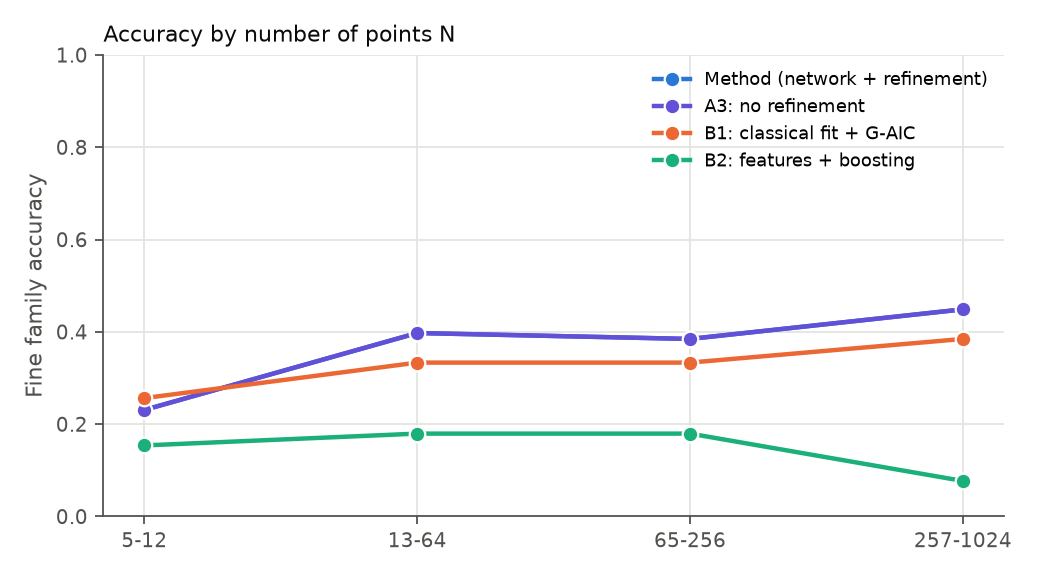
\includegraphics[width=0.48\textwidth]{fig_by_n.png}\hfill
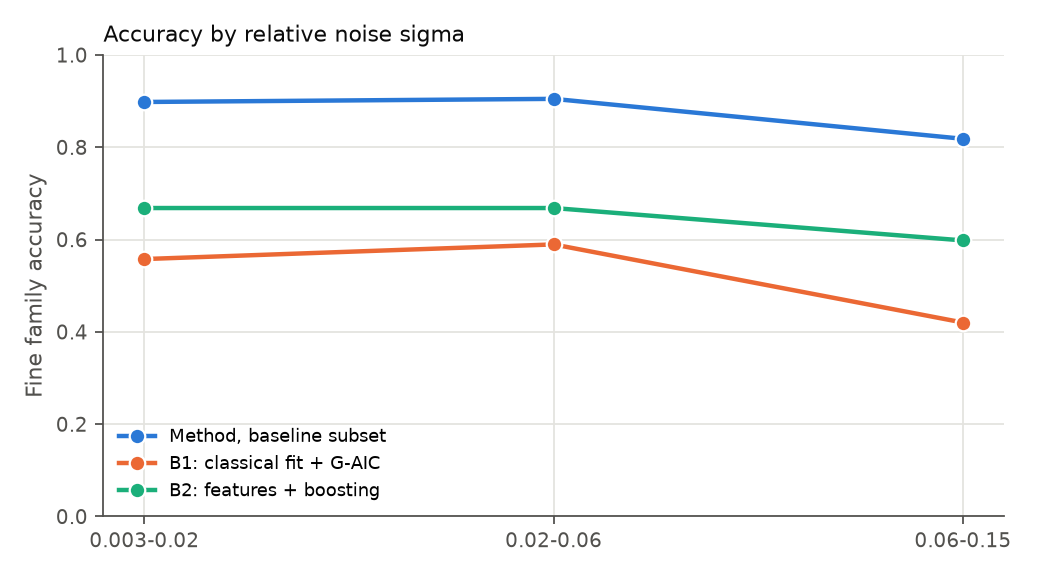
\includegraphics[width=0.48\textwidth]{fig_by_noise.png}
\caption{Fine accuracy by number of points and by relative noise on the baseline subset (the same clouds for every line). A3 is omitted because its accuracy equals the method's by construction.}
\label{fig:byn}
\end{figure}

\begin{figure}[tbp]
\centering
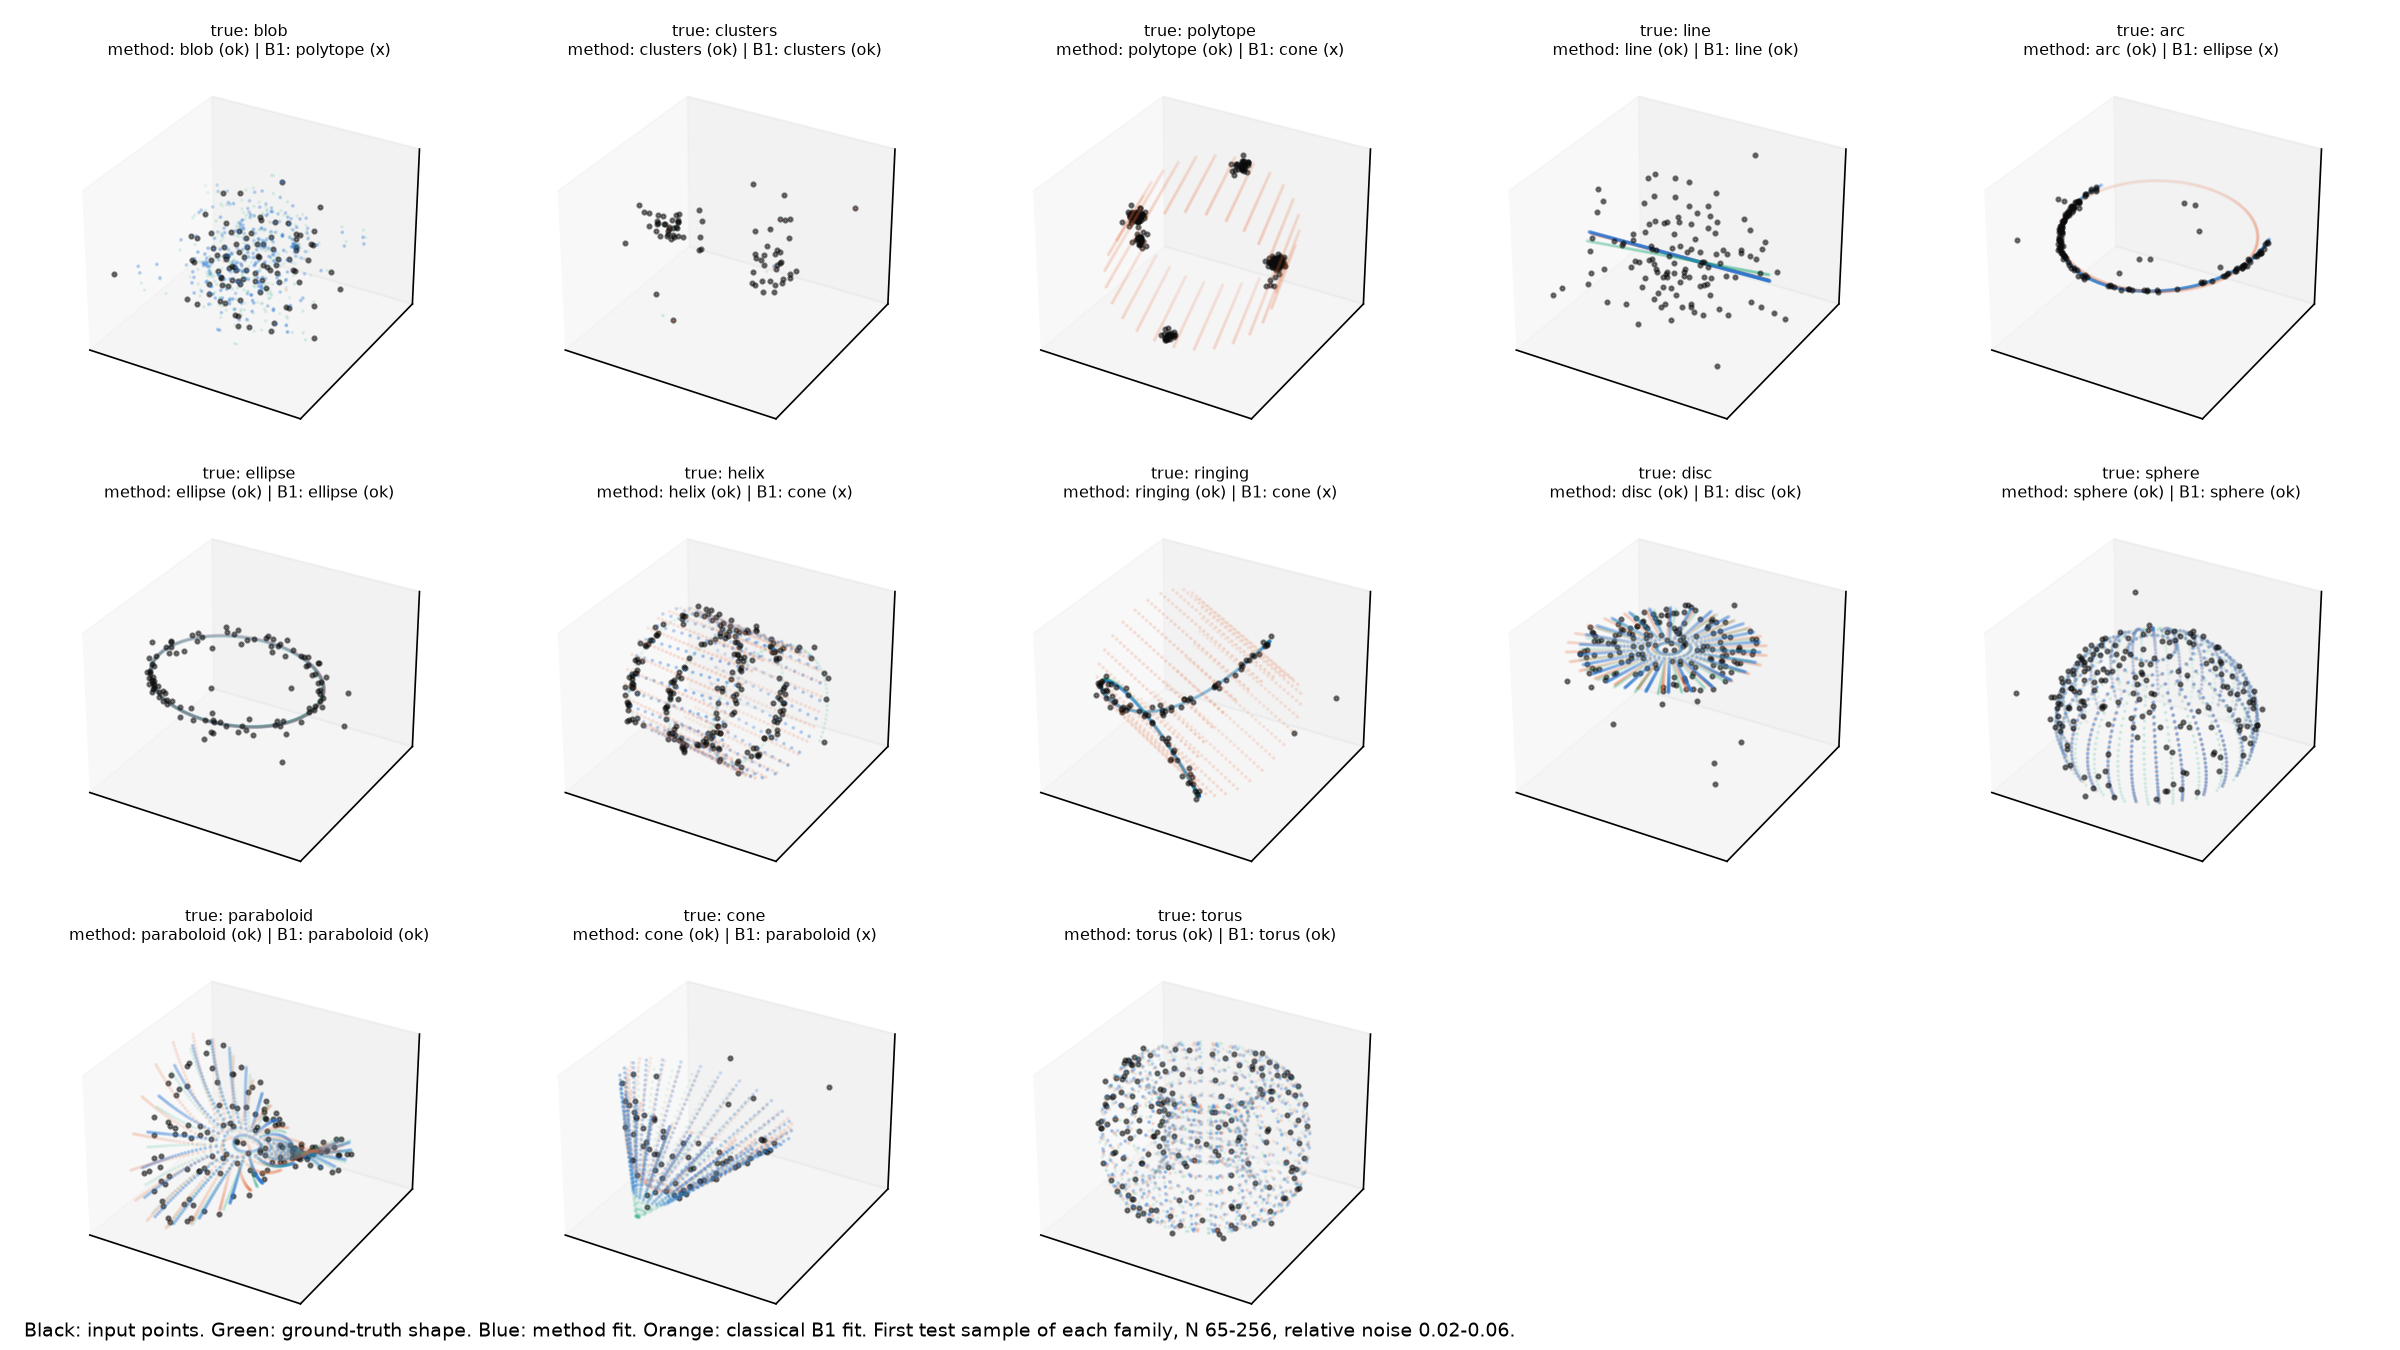
\includegraphics[width=\textwidth]{fig_gallery_synth.png}
\caption{The first synthetic test cloud of every family (65--256 points, relative noise 0.02--0.06): input points (black), ground-truth shape (green), method fit (blue), classical B1 fit (orange).}
\label{fig:gallery}
\end{figure}

\subsection{Real activations}
Table~\ref{tab:real} lists every real dataset and control, and Fig.~\ref{fig:real} shows the clouds with the fitted shapes. The coarse label agrees with the literature on \hthreeAgree{}/\hthreeN{} preregistered datasets; the label-permutation null gives $p=\hthreeP{}$, so \textbf{H3 is not supported} (it is not falsified either, since agreement is not below 50\%).

\paragraph{Successes.} The toy model of superposition with 6 features (R3) is labelled \fitRthreetmsnsix{} ($p=\pRthreetmsnsix{}$), with a fitted vertex on every feature direction (the octahedron of \citealp{elhage2022tms}). Llama's character-count manifold (R4) is labelled \fitRfourllamacounting{} ($p=\pRfourllamacounting{}$), a curve as in \citet{gurnee2025linebreaks}; under the preregistered rule a helix claim is not made because ringing is not rejected. Temperature (R8a) is labelled \fitReightallamatemperature{}, the arch PCA produces for a smoothly varying ordinal variable \citep{novembre2008horseshoe,antognini2018walks}, which agrees with the ``line'' of \citet{bhalla2026sae} at the coarse level. Colours (R7) are labelled \fitRsevenllamacolors{}, a curved surface as reported (paraboloid in \citealp{bhalla2026sae}).

\paragraph{Failures.} (i) GPT-2's positional embeddings (R1) are a 1D spiral whose radius varies along the curve; no family represents it (helix has constant radius, ringing three harmonics), and the classifier selects \fitRonegpttwowpos{} ($p=\pRonegpttwowpos{}$), a surface the spiral lies on. The held-out residual cannot reveal this error because held-out points also lie on the sphere. (ii) Weekdays and months (R5) form one tight cluster per token, 7 and 12 clusters, more than the 6 centroids the clusters family allows; the fitter threads a \fitRfiveallamaweekdays{} through them. (iii) Years (R6) and the grokked embeddings (R2) keep only \varRsixllamayears{} and \varRtwogrokkingWE{} of the variance in the top three components and are flagged ($\lambda_3/\lambda_4<1.5$): the 3D view cuts through a higher-dimensional structure, as expected for the several Fourier circles of a grokked model \citep{nanda2023progress}. (iv) Age (R8b) is a branching curve and true/false city statements (R9) two overlapping clouds of very different spread; both are outside the vocabulary (labelled \fitReightbllamaage{} and \fitRninellamatruthcities{}).

\begin{figure}[tbp]
\centering
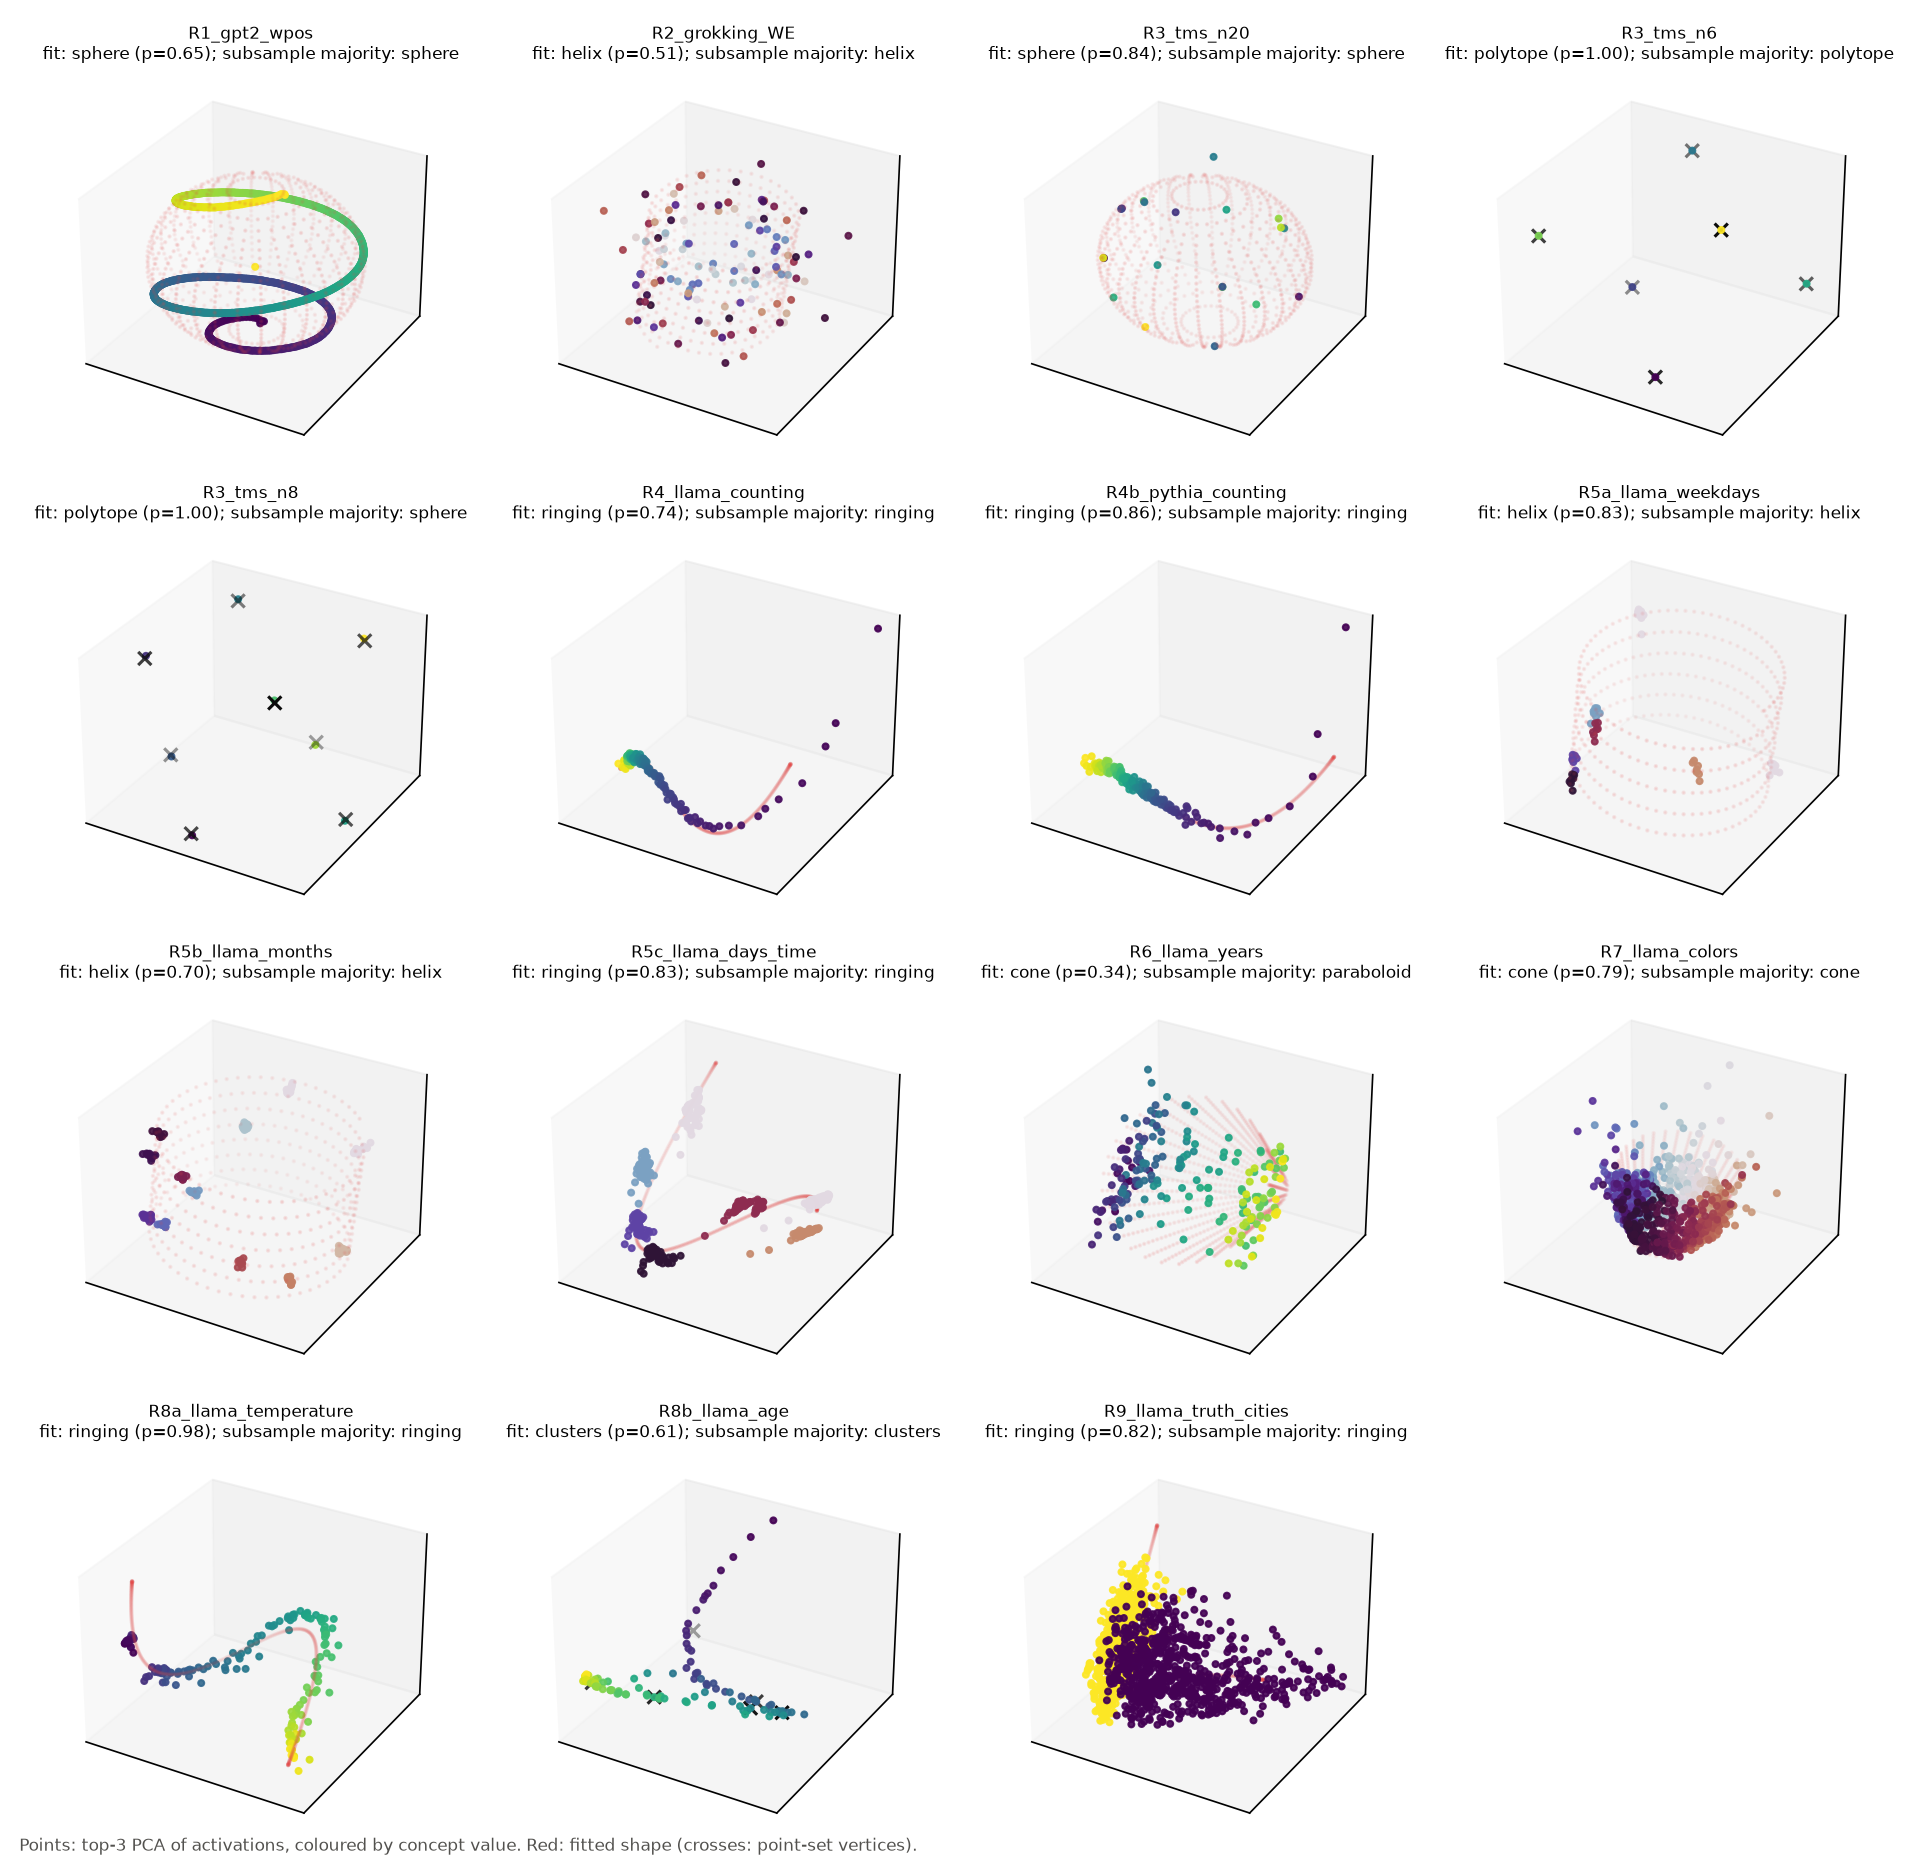
\includegraphics[width=\textwidth]{fig_real.png}
\caption{Real activation clouds in their top-3 PCA coordinates, coloured by concept value, with the fitted shape (red; crosses for point-set vertices). Titles give the full-cloud fit with its calibrated probability and the majority label over 200 random 80\% subsamples.}
\label{fig:real}
\end{figure}

\paragraph{Controls (H4).} Matched-covariance Gaussians are labelled blob in \hfourBlob{} of draws and the ordinal-process controls ringing in \hfourRing{} versus helix in \hfourHelix{}, so H4 passes as preregistered. A post-hoc split shows that this pass relies on the random walks (ringing in \hfourWalkRing{}): the smooth Gaussian-process controls alone are labelled helix in \hfourGpHelix{}. The classifier therefore confuses smooth ordinal processes with helices, the confound the preregistered helix rule guards against; for the fully evaluated Gaussian-process control the held-out residual favours ringing and the rule rejects the helix claim. Randomly initialised GPT-2 positional embeddings and grokking embeddings are labelled blob, but randomly initialised Llama is labelled \fitCthreellamamonthsinit{} for the month prompts: Fig.~\ref{fig:controls} shows genuine clusters, one per input token, because a random transformer still separates token identities. The preregistered expectation ``blob'' for this control was wrong, not the fitter.

\begin{figure}[tbp]
\centering
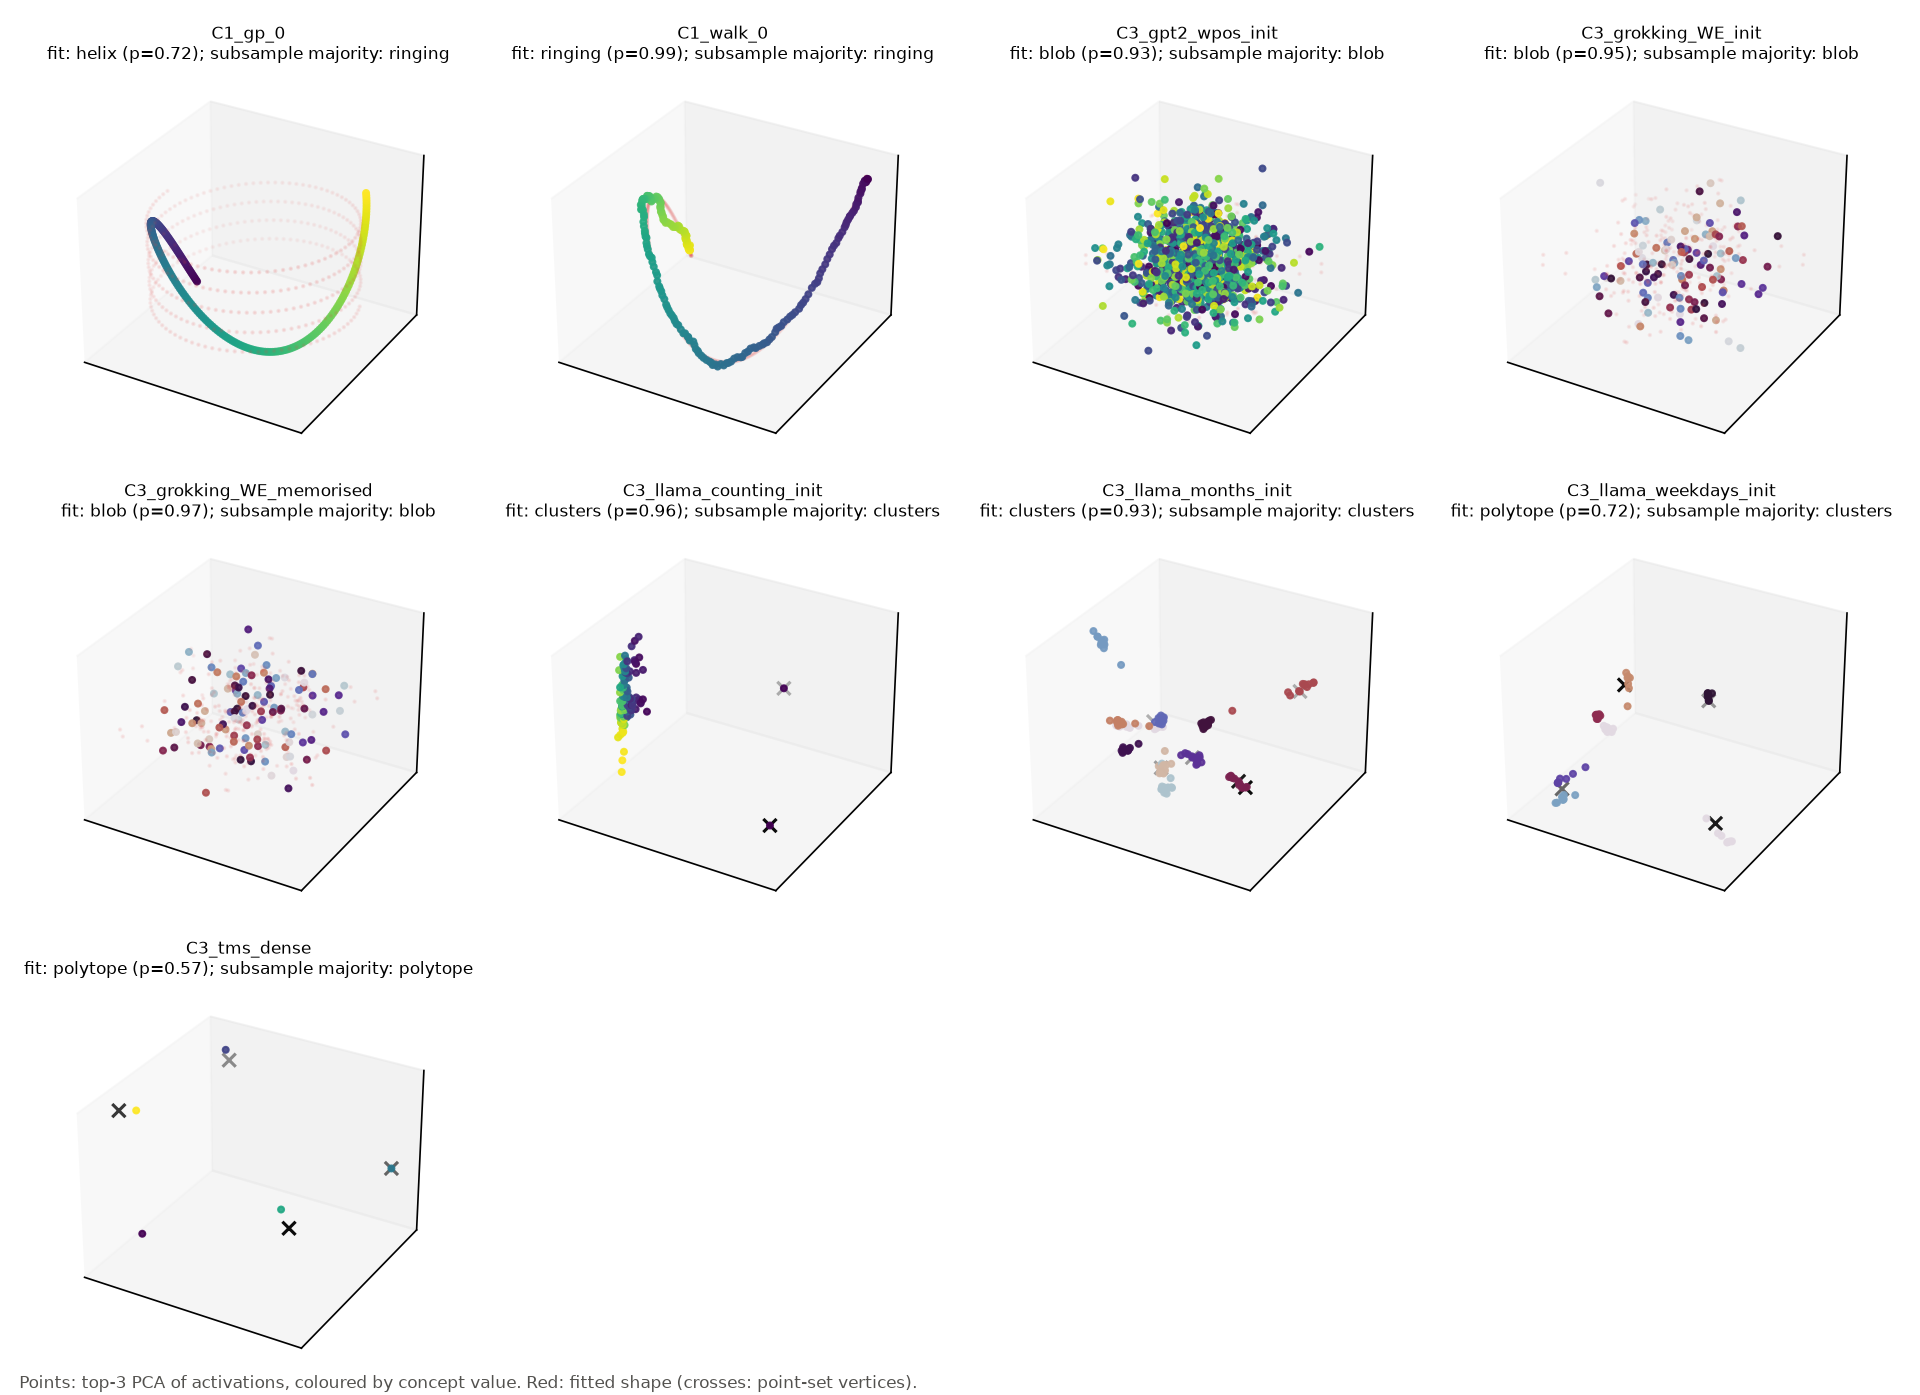
\includegraphics[width=\textwidth]{fig_controls.png}
\caption{Controls: a smooth Gaussian process and a random walk over an ordinal index (C1), and randomly initialised or untrained networks (C3).}
\label{fig:controls}
\end{figure}

\begin{sidewaystable}
\centering
\caption{Real datasets and controls (C1 shows the first of 10 draws of each process). Flags: $\lambda_3/\lambda_4<1.5$ (gap); OOD: residual above the synthetic 95th percentile of correct fits at that $N$. Held-out residuals, matched-Gaussian rates and model/layer details are in the full table in \texttt{reports/exp02\_real\_activations.md}.}
\label{tab:real}
\scriptsize
\begin{tabular}{llllllll}
\toprule
\textbf{Dataset} & \textbf{N x D} & \textbf{Top-3 var.} & \textbf{Expected (coarse / fine)} & \textbf{Fit (full cloud)} & \textbf{p} & \textbf{Subsample majority (freq.)} & \textbf{Flags} \\
\midrule
C1\_gp\_0 (prereg) & 200 x 768 & 99\% & 1d / ringing & helix & 0.72 & ringing (58\%) & - \\
C1\_walk\_0 (prereg) & 200 x 768 & 83\% & 1d / ringing & ringing & 0.99 & ringing (100\%) & - \\
C3\_gpt2\_wpos\_init (prereg) & 1023 x 768 & 1\% & 3d / blob & blob & 0.93 & blob (100\%) & gap$<$1.5 \\
C3\_grokking\_WE\_init (prereg) & 113 x 128 & 9\% & 3d / blob & blob & 0.95 & blob (100\%) & gap$<$1.5 \\
C3\_grokking\_WE\_memorised & 113 x 128 & 15\% & - / - & blob & 0.97 & blob (100\%) & gap$<$1.5 \\
C3\_llama\_counting\_init (prereg) & 150 x 4096 & 14\% & 3d / blob & clusters & 0.96 & clusters (98\%) & gap$<$1.5, OOD \\
C3\_llama\_months\_init (prereg) & 144 x 4096 & 19\% & 3d / blob & clusters & 0.93 & clusters (82\%) & gap$<$1.5, OOD \\
C3\_llama\_weekdays\_init (prereg) & 49 x 4096 & 34\% & 3d / blob & polytope & 0.72 & clusters (70\%) & gap$<$1.5, OOD \\
C3\_tms\_dense & 5 x 3 & 100\% & - / - & polytope & 0.57 & polytope (100\%) & - \\
R1\_gpt2\_wpos (prereg) & 1023 x 768 & 91\% & 1d / helix & sphere & 0.65 & sphere (74\%) & - \\
R2\_grokking\_WE (prereg) & 113 x 128 & 32\% & 1d / arc, ellipse & helix & 0.51 & helix (43\%) & gap$<$1.5 \\
R3\_tms\_n20 & 20 x 3 & 100\% & 0d / polytope, clusters & sphere & 0.84 & sphere (78\%) & - \\
R3\_tms\_n6 (prereg) & 6 x 3 & 100\% & 0d / polytope, clusters & polytope & 1.00 & polytope (100\%) & - \\
R3\_tms\_n8 (prereg) & 8 x 3 & 100\% & 0d / polytope, clusters & polytope & 1.00 & sphere (56\%) & - \\
R4\_llama\_counting (prereg) & 150 x 4096 & 69\% & 1d / helix & ringing & 0.74 & ringing (92\%) & - \\
R4b\_pythia\_counting & 150 x 1024 & 75\% & 1d / helix & ringing & 0.86 & ringing (100\%) & - \\
R5a\_llama\_weekdays (prereg) & 49 x 4096 & 66\% & 1d / arc & helix & 0.83 & helix (58\%) & gap$<$1.5 \\
R5a\_llama\_weekdays\_means (prereg) & 7 x 4096 & 78\% & 1d / arc & sphere & 0.40 & helix (74\%) & gap$<$1.5 \\
R5b\_llama\_months (prereg) & 144 x 4096 & 55\% & 1d / arc & helix & 0.70 & helix (87\%) & gap$<$1.5 \\
R5b\_llama\_months\_means (prereg) & 12 x 4096 & 60\% & 1d / arc & helix & 0.40 & helix (51\%) & gap$<$1.5 \\
R5c\_llama\_days\_time & 336 x 4096 & 58\% & 1d / arc & ringing & 0.83 & ringing (86\%) & gap$<$1.5 \\
R6\_llama\_years (prereg) & 199 x 4096 & 25\% & 1d / helix & cone & 0.34 & paraboloid (62\%) & gap$<$1.5 \\
R7\_llama\_colors (prereg) & 900 x 4096 & 66\% & 2d / paraboloid & cone & 0.79 & cone (83\%) & gap$<$1.5 \\
R8a\_llama\_temperature (prereg) & 150 x 4096 & 90\% & 1d / line & ringing & 0.98 & ringing (100\%) & - \\
R8b\_llama\_age (prereg) & 99 x 4096 & 85\% & 1d / line & clusters & 0.61 & clusters (96\%) & OOD \\
R9\_llama\_truth\_cities (prereg) & 1496 x 4096 & 53\% & 0d / clusters & ringing & 0.82 & ringing (100\%) & OOD \\
\bottomrule
\end{tabular}

\end{sidewaystable}


\section{Discussion and limitations}
% Discussion and limitations. Numbers are macros from generated/numbers.tex.

\paragraph{What the results support.} On synthetic clouds drawn from the 13-family generative model, a network trained only on synthetic data identifies the family and recovers the shape better than a classical pipeline that fits every family and selects with geometric AIC (H1, H2), and its probabilities are well calibrated after temperature scaling. This is a \emph{systematic} claim within the synthetic distribution (\nMethod{} test clouds over all point-count and noise bins), with paired bootstrap CIs. The ablation A5 attributes most of the advantage to model selection: given the same refined candidates, geometric AIC selects much worse than the learned classifier.

\paragraph{What the results do not support.} The fitter is not yet a reliable replacement for by-eye shape calls on real activations. Coarse agreement with the literature (H3) is not above a permutation null. Post-hoc inspection suggests causes for the coarse misses: a curve outside the vocabulary (GPT-2 positions), a top-3 projection of higher-dimensional structure (years), clouds unlike any training family (age, true/false statements) and an unstable label on an 8-point cloud. At the fine level, more than six discrete groups (weekdays, months) are threaded with a helix. These explanations were not tested. In each case the classifier still returns a confident label, because a closed-set classifier must pick one of its 13 families. Smooth ordinal controls are frequently labelled helix (\hfourGpHelix{} of the Gaussian-process controls, post hoc), so a helix label from the classifier alone is not evidence of a helix. The preregistered two-part rule (probability ratio and held-out residual) is necessary but not sufficient: it rejected the helix claim for the Gaussian-process control but accepted it for \helixRuleAccepted{}, which the literature describes as circles.

\paragraph{Implications for practice.} (1) Report the shape of the top-3 projection together with the explained variance and the $\lambda_3/\lambda_4$ gap; a low gap means the 3D picture is a slice. (2) Treat ``helix'' as a hypothesis to be tested with held-out data against the PCA ringing artifact \citep{novembre2008horseshoe,antognini2018walks,shinn2023phantom} and against discrete clusters or a circle. (3) Controls with random weights are not structureless when inputs differ in token identity; a token-identity-matched control is the right null for prompt-based datasets. (4) Exclude sequence position 0 (BOS or the first token) when averaging activations: the starting token carries massive activations and attracts attention as a sink \citep{sun2024massive,xiao2024sinks}, which can dominate class means.

\paragraph{Limitations.}
\label{sec:limitations}
\begin{itemize}
\item \textbf{One seed, no trained ablations yet.} All results come from one trained model (\texttt{main\_s0}); the seed, learning-rate and inference-hyperparameter sweeps and the trained ablations A1, A2, A4, A6 (including H5a) are implemented but postponed to later stages (\texttt{reports/deviations.md}). Synthetic CIs therefore reflect test-sample variation only, not training variation.
\item \textbf{Baselines on a subset.} B1 and B2 were run on 20 clouds per family and cell (\nBone{} clouds) because B1 runs 61 refinements per cloud; all paired comparisons use this subset.
\item \textbf{Closed vocabulary.} 13 families with label margins between nested families; shapes outside the vocabulary are forced into one of them. There is no abstention beyond the OOD and gap flags.
\item \textbf{Synthetic prior.} Training data follow hand-designed families and nuisances; real activation clouds differ (non-uniform density along curves, token-level clusters, outliers), which is the main source of the synthetic-to-real gap.
\item \textbf{Top-3 PCA only.} All statements concern the top-3 projection, as the task specifies; intrinsic manifolds can differ, and causal roles of these representations are not tested.
\item \textbf{Literature labels as ground truth.} H3 compares against published descriptions that were themselves made by eye, often with different models, layers or prompts (we use Llama-3.1-8B for all preregistered LLM datasets). The grokked model was trained for fewer epochs than in \citet{nanda2023progress}, and one weekday prompt differs by one word from \citet{engels2025notall}.
\end{itemize}


\section{Conclusion}
% Conclusion. Numbers are macros from generated/numbers.tex.
We built a catalog of empirically reported neural geometries, a 13-family shape vocabulary with unique canonical parameters, and a Set Transformer that maps a top-3 PCA point cloud to a family and its parameters, trained only on synthetic shapes with a shape-to-shape Chamfer loss. On held-out synthetic data it identifies the family in \accMethod{} of clouds and beats a classical fit-every-family pipeline with geometric-AIC selection on both family identification and shape recovery (H1, H2 supported). On real activations, coarse agreement with published shape descriptions (\hthreeAgree{}/\hthreeN{}) is not above a permutation null (H3 not supported), and controls show that smooth ordinal processes are often mistaken for helices. The failure modes suggested by post-hoc inspection---out-of-vocabulary curves, many discrete groups, unequal clusters and low-variance projections---point to the next steps: a coverage check that penalises fitted shapes without supporting points, a more flexible Fourier-curve family, more cluster centroids, a helix test against circles and clusters as well as ringing, and abstention for clouds outside the training distribution.


\section*{Reproducibility}
All code (MIT license), configurations, results files, the preregistration and the deviation log are at \url{https://github.com/BurnyCoder/geometrical-shape-fitting-in-llm-mechanistic-interpretability}. One command (\texttt{uv run python run.py report --config main.yaml}) regenerates every number, table and figure in this paper from the results files. The trained fitter and the run logs (training, evaluation, and activation extraction with every LLM prompt) are on the Hugging Face Hub at \url{https://huggingface.co/BurnyCoder/neurogeom-shape-fitter-main-s0} (collection ``Fitting geometric shapes to neural geometry''), and an interactive explorer of all fits is at \url{https://burnycoder.github.io/geometrical-shape-fitting-in-llm-mechanistic-interpretability/}.

\bibliographystyle{plainnat}
\bibliography{references}

\appendix
\section{Catalog of empirically reported shapes}
\label{app:catalog}
{\scriptsize
\begin{tabular}{p{3.2cm}p{3.2cm}p{3.3cm}p{1.5cm}p{1.4cm}p{3.2cm}}
\toprule
\textbf{Shape} & \textbf{Concept} & \textbf{Model / layer} & \textbf{Top-3 PCA} & \textbf{Family} & \textbf{Source} \\
\midrule
circle (overall a cone; PC1 = intensity/radius) & days of the week, months of the year (also 20th-century years in GPT-2) & GPT-2-small L7 (SAE clusters); Mistral-7B L8/L30; Llama-3-8B L5 & yes (PCs 1-2 or 2-3) & arc & \href{https://arxiv.org/abs/2405.14860}{Engels et al. 2024/2025, Not All Language Model Features Are} \\
circle ("days of the week organized in a cycle") & days of the week (prompt "It's {time} on day") & Llama-3.1-8B L19, last token & yes & arc & \href{https://arxiv.org/abs/2604.28119}{Bhalla et al. 2026, Do Sparse Autoencoders Capture Concept M} \\
circles (one per key Fourier frequency, "clock") & residues in modular addition (a+b mod p) & 1-layer transformer trained from scratch, p=113 / p=59 & yes (PCs 1-2; PC3 belongs to another frequency) & arc & \href{https://arxiv.org/abs/2301.05217}{Nanda et al. 2023, Progress measures for grokking via mechan} \\
ring / square grid / hexagonal lattice (in-context graph structure) & graph defined in context by random walks over tokens & Llama-3.1-8B L26 & yes (top-2 PCs) & arc & \href{https://arxiv.org/abs/2501.00070}{C. F. Park et al. 2025, ICLR: In-Context Learning of Represe} \\
circle (valence-arousal circumplex) & emotions & Llama-3.1-8B, Qwen3-8B/14B & yes (2D) & arc & \href{https://arxiv.org/abs/2604.03147}{Sun et al. 2026, Valence-Arousal Subspace in LLMs: Circular } \\
ring & head direction (neuroscience analogue) & mouse anterodorsal thalamic nucleus & yes & arc & \href{https://doi.org/10.1038/s41593-019-0460-x}{Chaudhuri, Gercek, Pandey, Peyrache, Fiete 2019, The intrins} \\
helix & learned absolute positional embeddings (W\_pos, 1024 x 768) & GPT-2 small/medium/large (weak in XL) & yes (~90\% variance in 3 PCs for GPT-2 small) & helix & \href{https://www.lesswrong.com/posts/qvWP3aBDBaqXvPNhS/gpt-2-s-positional-embedding-matrix-is-a-helix}{Yedidia 2023, GPT-2's positional embedding matrix is a helix} \\
twisting helix-like rippled curve (1D manifold in ~6D) & character count since last line break & Claude 3.5 Haiku L2; replicated in Llama-3.1-8B L5 / Qwen3-8B L5 (PC1-3 = 97\% variance) & yes & helix & \href{https://transformer-circuits.pub/2025/linebreaks/index.html}{Gurnee et al. 2025, When Models Manipulate Manifolds: The Ge} \\
generalized helix (line + circles with periods 2, 5, 10, 100) & integers 0-360 & GPT-J, Pythia-6.9B, Llama-3.1-8B (residual after layer 0) & partial (PC1 ~ linear; helix only in fitted subspace) & helix & \href{https://arxiv.org/abs/2502.00873}{Kantamneni \& Tegmark 2025, Language Models Use Trigonometry } \\
helix & years (prompt "The date is year") & Llama-3.1-8B L19, last token & unknown (not plotted) & helix & \href{https://arxiv.org/abs/2604.28119}{Bhalla et al. 2026, Do Sparse Autoencoders Capture Concept M} \\
periodic Fourier features (circles per digit/period) & numbers in addition & pre-trained LLMs (GPT-2 family and others) & unknown & arc & \href{https://arxiv.org/abs/2406.03445}{Zhou et al. 2024, Pre-trained Large Language Models Use Four} \\
line & temperature ("Today it's {f} degrees Fahrenheit outside"), age ("They are {age} years old."), formality, sentence length & Llama-3.1-8B L19, last token & yes (Fig. 2) & line & \href{https://arxiv.org/abs/2604.28119}{Bhalla et al. 2026, Do Sparse Autoencoders Capture Concept M} \\
line / linear map (latitude, longitude, year) & places and historical entities & Llama-2 7B/13B/70B, mid-depth & no (top PCs separate entity types) & line & \href{https://arxiv.org/abs/2310.02207}{Gurnee \& Tegmark 2024, Language Models Represent Space and T} \\
sphere (cities); circle (dates, time of day); semicircle (events 1900-2000); log-line (durations); clusters (seasons) & time and space concepts & Llama-3.x, Qwen2.5, Gemma-2 & no (paper: PCA misses subspaces not aligned with max variance) & sphere & \href{https://arxiv.org/abs/2510.01025}{Tiblias et al. 2025 (TMLR 2026), Hypothesis-Driven Feature M} \\
paraboloid ("circular hue and lightness dimensions") & colors (prompt "The hex code {h\_code} is for the color") & Llama-3.1-8B L19, last token & yes (Fig. 2) & paraboloid & \href{https://arxiv.org/abs/2604.28119}{Bhalla et al. 2026, Do Sparse Autoencoders Capture Concept M} \\
disc ("pizza") or torus in first layer; circle in later layers & modular addition & small MLPs and transformers trained from scratch & disc yes; torus needs 4D & torus & \href{https://arxiv.org/abs/2512.25060}{Moisescu-Pareja et al. 2025, On the geometry and topology of} \\
filled disc ("pizza") of embeddings & residues in modular addition (pizza algorithm, attention-rate-dependent) & 1-layer transformers trained from scratch & yes (PCs 1-2) & disc & \href{https://arxiv.org/abs/2306.17844}{Zhong, Liu, Tegmark, Andreas 2023, The Clock and the Pizza: } \\
torus & grid-cell modules (neuroscience analogue) & rat medial entorhinal cortex & no (needs 4D) & torus & \href{https://doi.org/10.1038/s41586-021-04268-7}{Gardner et al. 2022, Toroidal topology of population activit} \\
narrow cone (anisotropy) & all contextual embeddings & GPT-2, BERT, ELMo & partial (PC1 dominance) & cone & \href{https://arxiv.org/abs/1909.00512}{Ethayarajh 2019, How Contextual are Contextualized Word Repr} \\
two linearly separated clusters & true vs false statements & LLaMA-13B (and LLaMA-2 family) & yes & clusters & \href{https://arxiv.org/abs/2310.06824}{Marks \& Tegmark 2024, The Geometry of Truth} \\
antipodal pairs, triangles, pentagons, tetrahedra, square antiprisms & features in superposition & toy ReLU autoencoders & n/a (weights are already low-dimensional) & polytope & \href{https://transformer-circuits.pub/2022/toy_model/index.html}{Elhage et al. 2022, Toy Models of Superposition} \\
simplices / polytopes; hierarchy orthogonal & WordNet categories & Gemma, LLaMA-3 & no & polytope & \href{https://arxiv.org/abs/2406.01506}{K. Park, Choe, Jiang, Veitch 2024, The Geometry of Categoric} \\
parallelogram "crystals", lobes & SAE decoder directions & (SAE features of LLMs) & no & polytope & \href{https://arxiv.org/abs/2410.19750}{Li, Michaud, Baek, Engels, Sun, Tegmark 2025, The Geometry o} \\
hierarchical tree & geographical coordinates $\to$ country & Llama-3.1-8B L19 & unknown & out-of-vocab & \href{https://arxiv.org/abs/2604.28119}{Bhalla et al. 2026} \\
fractal inside a 2-simplex & belief states of a hidden Markov process (Mess3) & 4-layer transformer, d=64 & no & out-of-vocab & \href{https://arxiv.org/abs/2405.15943}{Shai et al. 2024, Transformers represent belief state geomet} \\
Klein bottle & 3x3 natural image patches (and reportedly first-layer CNN filters) & natural image statistics; CNNs (secondary claim) & no (needs 4D) & out-of-vocab & \href{https://link.springer.com/article/10.1007/s11263-007-0056-x}{Carlsson et al. 2008, On the Local Behavior of Spaces of Nat} \\
circle of rotating edge filters & first-layer convolution filters & CNNs on MNIST, CIFAR-10, SVHN, ImageNet & n/a & arc & \href{https://arxiv.org/abs/1810.03234}{Bruel Gabrielsson \& Carlsson 2018, Exposition and Interpreta} \\
nested "onion" shells (magnitude-coded position) & sequence position & gated RNNs (GRUs) & no & out-of-vocab & \href{https://arxiv.org/abs/2408.10920}{Csordas et al. 2024, Recurrent Neural Networks Learn to Stor} \\
\bottomrule
\end{tabular}}

\section{Additional results}
% Appendix: additional generated tables and figures.

\subsection{Unambiguous synthetic subset}
Synthetic clouds that a simpler family also fits equally well (judged from B1's per-family fits) are tagged ambiguous (\ambiguousFrac{} of the baseline subset). Table~\ref{tab:unambiguous} repeats Table~\ref{tab:results} without them.
\begin{table}[H]
\centering
\caption{Systems on the baseline subset without ambiguous clouds.}
\label{tab:unambiguous}
\resizebox{\textwidth}{!}{\scriptsize
\begin{tabular}{lllllllll}
\toprule
\textbf{System} & \textbf{n} & \textbf{Fine accuracy [95\% CI]} & \textbf{Macro-F1 [95\% CI]} & \textbf{Coarse accuracy} & \textbf{Superset-OK accuracy} & \textbf{Median Chamfer to GT [95\% CI]} & \textbf{Mean residual} & \textbf{Median axis error (deg)} \\
\midrule
Method (network + refinement) & 2060 & 94.0\% [93.0, 95.0] & 0.922 [0.908, 0.935] & 96.4\% & 94.3\% & 0.119 [0.111, 0.127] & 0.091 & 0.7 \\
A3: no refinement & 2060 & 94.0\% [93.0, 95.0] & 0.922 [0.908, 0.935] & 96.4\% & 94.3\% & 0.127 [0.119, 0.132] & 0.101 & 1.1 \\
A5: G-AIC selection & 2060 & 72.0\% [70.1, 74.0] & 0.654 [0.637, 0.671] & 81.5\% & 76.5\% & 0.138 [0.134, 0.144] & 0.097 & 0.6 \\
A5: hybrid selection & 2060 & 92.6\% [91.4, 93.7] & 0.902 [0.888, 0.916] & 94.8\% & 93.1\% & 0.119 [0.111, 0.128] & 0.090 & 0.7 \\
B1: classical fit + G-AIC & 2060 & 69.7\% [67.6, 71.6] & 0.636 [0.615, 0.654] & 82.5\% & 75.4\% & 0.154 [0.147, 0.160] & 0.103 & 0.6 \\
B2: features + boosting & 2060 & 72.3\% [70.3, 74.2] & 0.697 [0.674, 0.715] & 92.5\% & 76.2\% & 0.152 [0.147, 0.159] & 0.099 & 0.6 \\
B3a: always blob & 2060 & 4.5\% [3.6, 5.4] & 0.007 [0.005, 0.008] & 4.5\% & 4.5\% & 0.523 [0.517, 0.529] & 0.119 & 10.2 \\
B3b: always arc (B1 arc fit) & 2060 & 7.3\% [6.2, 8.5] & 0.011 [0.009, 0.012] & 36.3\% & 7.3\% & 0.528 [0.516, 0.538] & 0.273 & 0.3 \\
B3c: random shape & 2060 & 8.3\% [7.2, 9.5] & 0.079 [0.068, 0.090] & 34.1\% & 11.6\% & 1.114 [1.092, 1.138] & 0.582 & 58.6 \\
\bottomrule
\end{tabular}
}
\end{table}

\subsection{Training, confusion and calibration}
\begin{figure}[H]
\centering
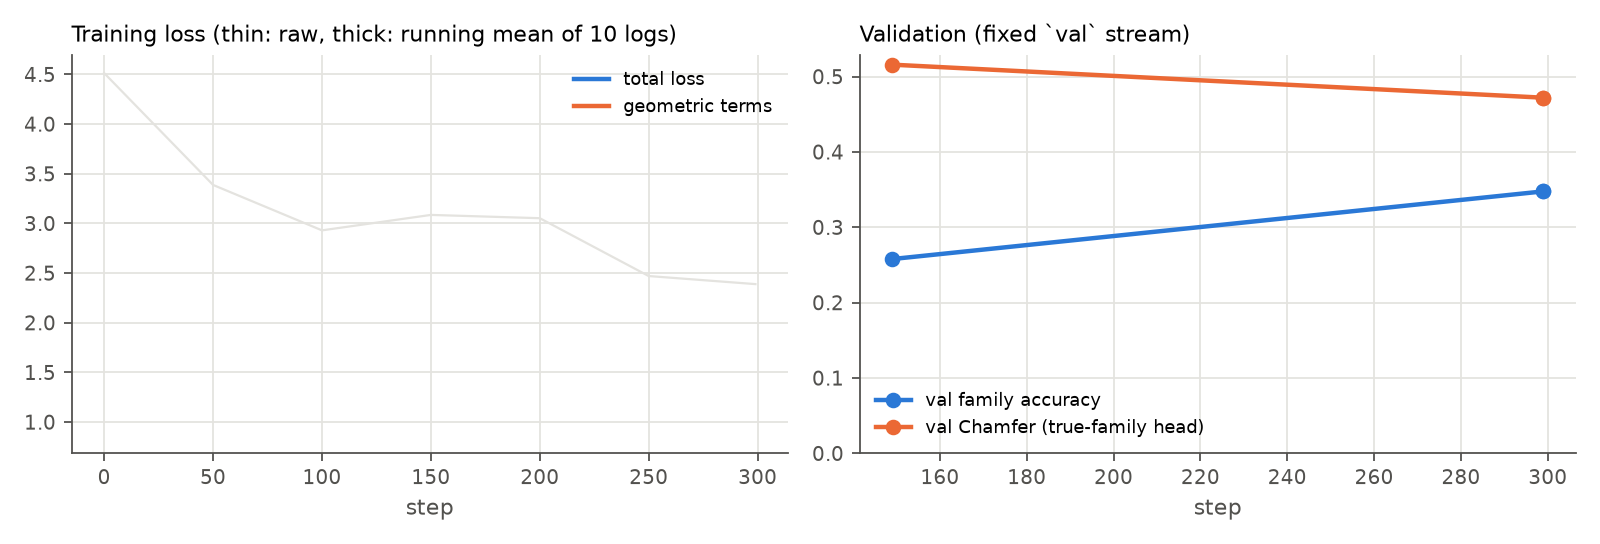
\includegraphics[width=\textwidth]{fig_training.png}
\caption{Training loss (left) and validation family accuracy and teacher-forced Chamfer distance on the fixed validation stream (right). Steps 0--9999 of the loss curve were recovered from the log of the crashed first attempt (\texttt{reports/deviations.md}).}
\label{fig:training}
\end{figure}
\begin{figure}[H]
\centering
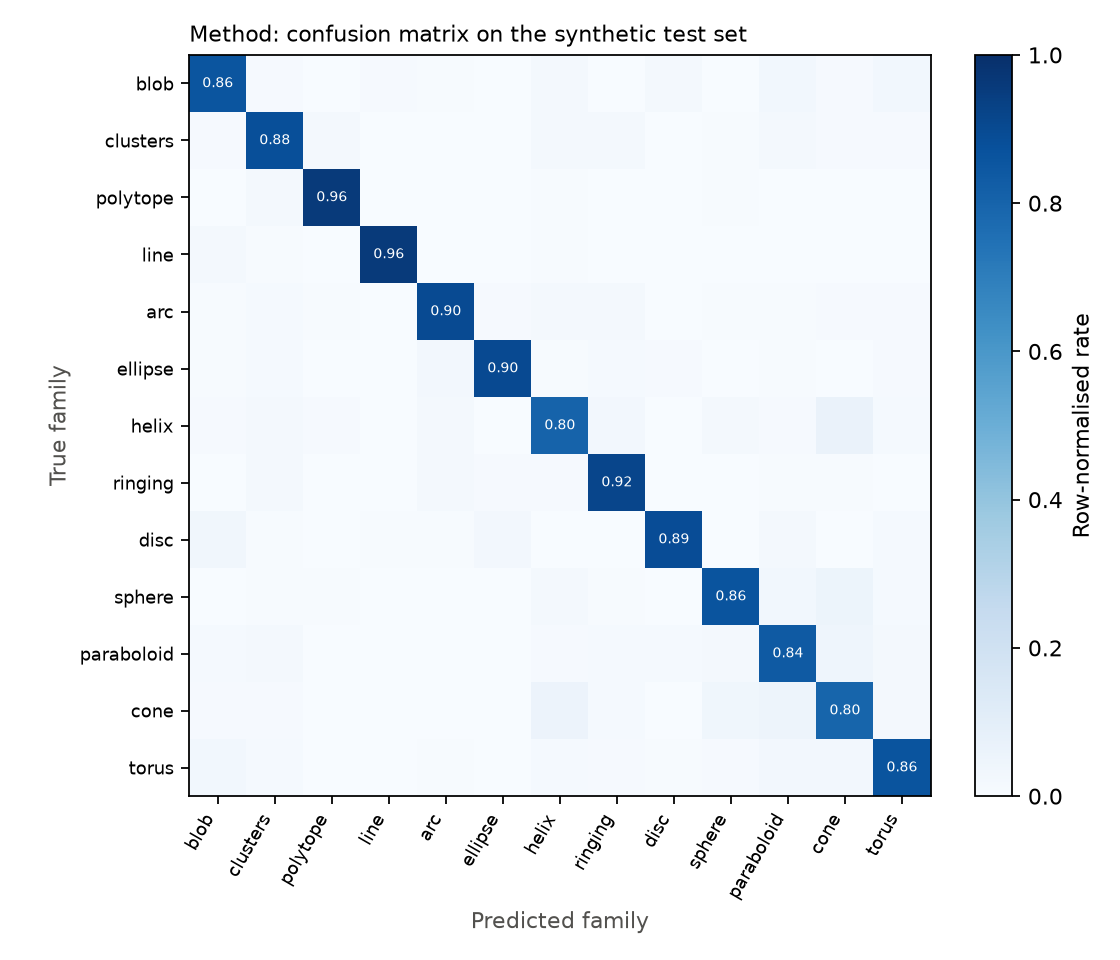
\includegraphics[width=0.55\textwidth]{fig_confusion.png}\hfill
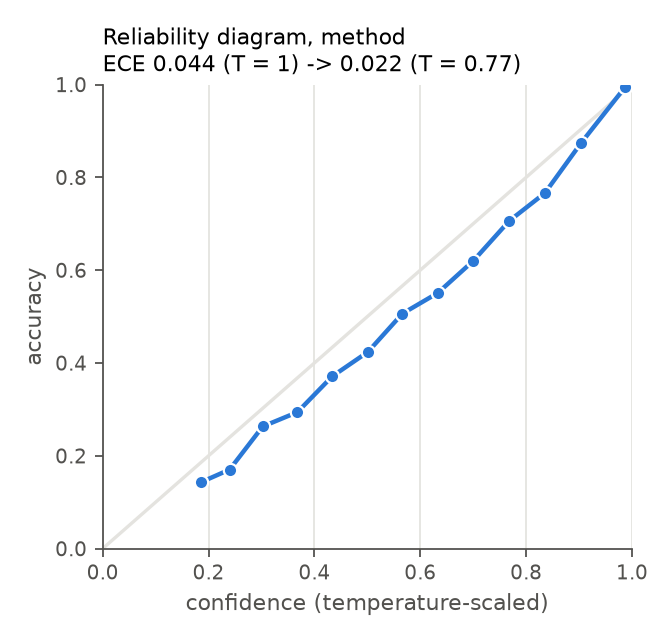
\includegraphics[width=0.4\textwidth]{fig_reliability.png}
\caption{Left: confusion matrix of the method on the full synthetic test set (row-normalised). Right: reliability diagram after temperature scaling.}
\label{fig:confusion}\label{fig:reliability}
\end{figure}
\begin{figure}[H]
\centering
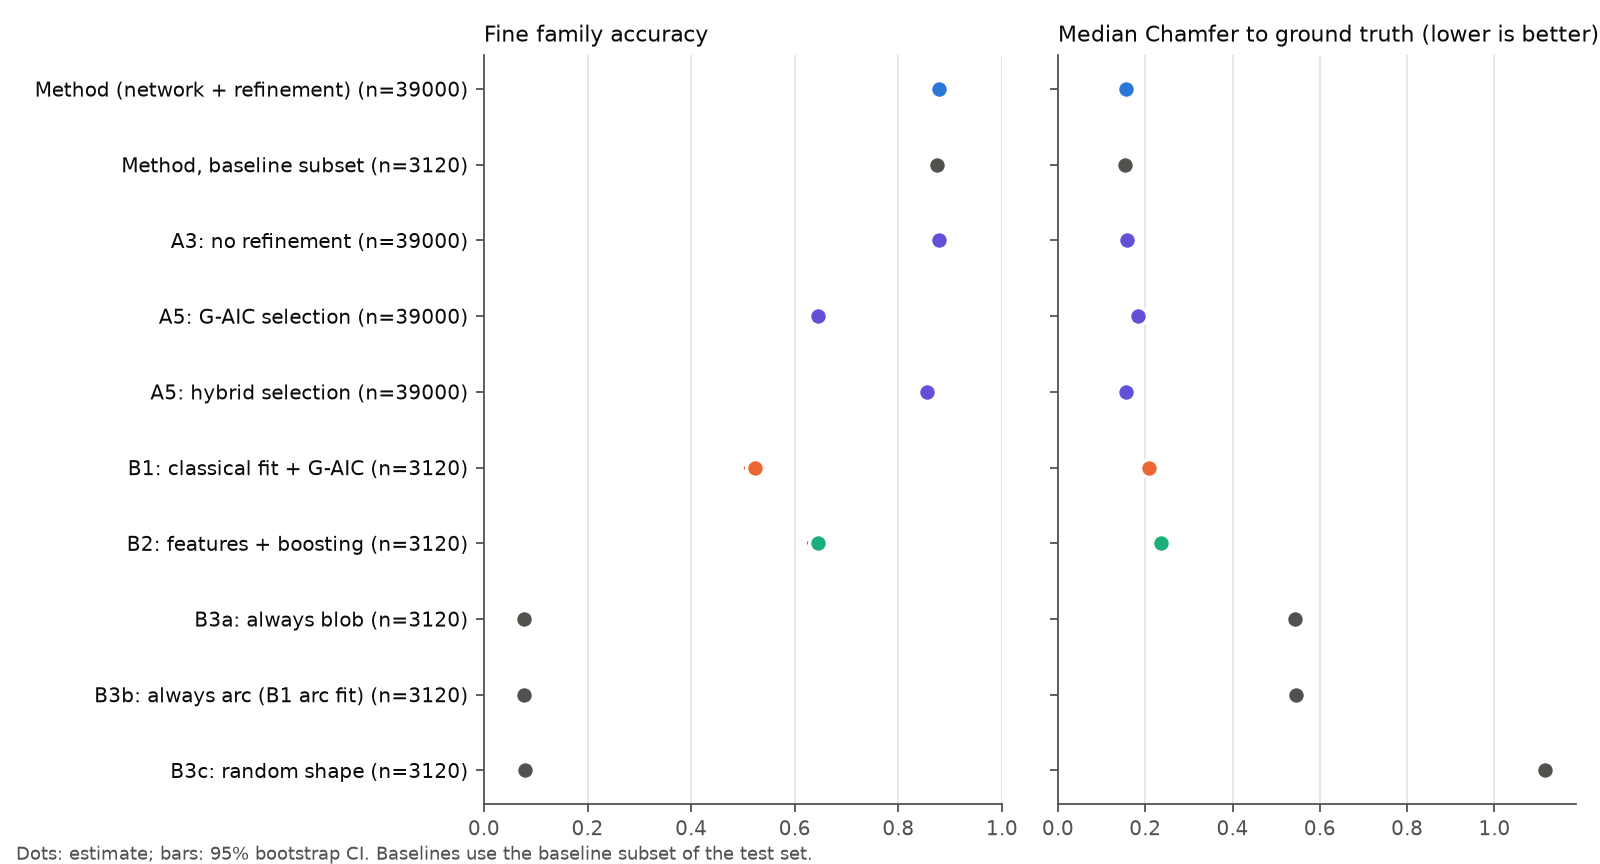
\includegraphics[width=\textwidth]{fig_systems.png}
\caption{Fine accuracy and median Chamfer distance of all systems with 95\% bootstrap CIs.}
\label{fig:systems}
\end{figure}

\subsection{Models}
\begin{table}[H]
\centering
\caption{Trained fitters.}
\resizebox{\textwidth}{!}{\scriptsize
\begin{tabular}{llllllllll}
\toprule
\textbf{Run} & \textbf{Encoder} & \textbf{Training objective} & \textbf{Data / curriculum} & \textbf{Params} & \textbf{Steps} & \textbf{Minutes} & \textbf{Val. accuracy} & \textbf{Test fine accuracy} & \textbf{Test median Chamfer} \\
\midrule
main\_s0 & Set Transformer & CE + Chamfer + residual + aux & full synthetic mix & 1,712,093 & 22643 & 110 & 90.2\% & 87.9\% & 0.156 \\
\bottomrule
\end{tabular}
}
\end{table}


\section*{AI statement}
This codebase and paper were written by Claude Code (Anthropic), an AI coding agent, which executed a specification provided by the human author; the human author provided the research question, constraints and standards to follow. Human cleanup and rewriting are in progress.
\end{document}
